\section{Motivating Example}\label{motivExample}

Suppose that you are student in a School of Magic.
It is your first day in the School, so navigation in the building is a problem for you.
Fortunately, you have a map of the building (fig.~\ref{input}) and an additional knowledge about building construction:
\begin{itemize}
  \item there are towers in the school (nodes of the graph in your map);
  \item all floors of some towers connected by directed galleries (edges in your map);
  \item each gallery has a ``magic'' property: start floor is aways one more (edge label is 'b') or one less (edge label is 'b') then end floor. 
\end{itemize}

\begin{figure}[h]
    \begin{center}
        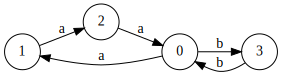
\includegraphics[width=6cm]{dot/input.pdf}
        \caption{The map of School (input graph $M$)}
        \label{input}        
    \end{center}
\end{figure}


You want to find a path from your current position to the same floor in another tower. 
Map with all such paths can help you.
But orienteering is not your forte, so it would be great if the structure of the paths were as simple as possible and all paths will have checkpoints to control your rout.

It is evident that the simplest structure of required paths is $\{ab, aabb, aaabbb, \dots\}$.
In terms of our definitions you have a graph $M=(\{0;1;2;3\},E,\{a;b\})$ (figure~\ref{input}), and you want to find all paths $p$, such that $\Omega(p) \in \{ab; aabb; aaabbb; \dots\}$ or $\Omega(p) \in a^n b^n$ where $n \geq 1$.


Unfortunately, language $\mathcal{L} = \{a^n b^n; n \geq 1\}$ is not regular which restricts the set of tools you can use. 
Another problem is the infinite size of solution, but you want to get a finite map.  
Moreover, you want to know a structure of paths with checkpoints added.

We are not aware of any existing tools which can help to solve this problem and we create a new one.
Let us to show how to get the map which help to orient in this strange School.

Fortunately, the language $\mathcal{L} = \{a^n b^n; n \geq 1\}$ is a context-free language and can be specified with context-free grammar. 
The fact that one language can be described with more than one grammar allows to add checkpoints: additional nonterminals can mark required parts of a sentence.
In our case, a desired checkpoint can be in the middle of the path.
As a result, required language can be specified by the grammar $G_1$ presented in figure~\ref{grammarG}, where $N = \{s; \text{\textit{Middle}}\}$, $\Sigma = \{a; b\}$, and $S$ is a start nonterminal.

\begin{figure}[h]
   \begin{center}
   \[
\begin{array}{rl}
   0:& S \rightarrow a \ S \ b \\
   1:& S \rightarrow Middle \\
   2:& Middle \rightarrow a \ b
\end{array}
\]

   \caption{Grammar $G_1$ for language $L=\{a^n b^n; n \geq 1\}$ with additional marker for a middle of a path}
   \label{grammarG}        
   \end{center}
\end{figure}

In the next section we present a map construction algorithm,  which solves such problems.
